\documentclass[11pt]{article}

\usepackage[margin=1in]{geometry}
\usepackage[T1]{fontenc}
\usepackage{graphicx}
\usepackage{longtable}
\usepackage{booktabs}
\usepackage{array}
\usepackage{ragged2e}
\usepackage{enumitem}
\usepackage{xcolor}
\usepackage{hyperref}
\usepackage{tikz}
\usepackage{float}
\usepackage{fancyhdr}
\usepackage{titlesec}
\usepackage{tcolorbox}
\usepackage{tabularx}
\usepackage{multirow}
\usepackage{caption}
\usepackage{listings}
\usepackage{makecell}
\usepackage{amssymb}
\usepackage{pifont}

\usetikzlibrary{shapes.geometric, arrows.meta, positioning, fit, backgrounds, calc, decorations.pathreplacing, shapes.multipart, matrix, shadows, mindmap}

% ---------------------------------------------------------------------------
% Color Definitions
% ---------------------------------------------------------------------------
\definecolor{sectionblue}{RGB}{31,78,121}
\definecolor{stakeholdercolor}{RGB}{70,130,180}
\definecolor{concerncolor}{RGB}{60,179,113}
\definecolor{viewcolor}{RGB}{255,165,0}
\definecolor{flowcolor}{RGB}{100,100,100}
\definecolor{lightgray}{RGB}{245,245,245}
\definecolor{warningred}{RGB}{220,53,69}
\definecolor{successgreen}{RGB}{40,167,69}
\definecolor{infoblue}{RGB}{23,162,184}
\definecolor{decisioncolor}{RGB}{186,85,211}
\definecolor{externalcolor}{RGB}{255,193,7}
\definecolor{technicalcolor}{RGB}{144,238,144}
\definecolor{businesscolor}{RGB}{255,182,193}
\definecolor{qualitycolor}{RGB}{173,216,230}

\hypersetup{
  colorlinks=true,
  linkcolor=sectionblue,
  urlcolor=sectionblue,
  citecolor=sectionblue
}

% ---------------------------------------------------------------------------
% Header and Footer
% ---------------------------------------------------------------------------
\pagestyle{fancy}
% Fix fancyhdr headheight warning
\setlength{\headheight}{14pt}
\addtolength{\topmargin}{-2pt}
\fancyhf{}
\fancyhead[L]{\leftmark}
\fancyhead[R]{Stakeholders and Concerns Guide}
\fancyfoot[C]{\thepage}
\renewcommand{\headrulewidth}{0.4pt}
\renewcommand{\footrulewidth}{0.4pt}

% ---------------------------------------------------------------------------
% Section Formatting
% ---------------------------------------------------------------------------
\titleformat{\section}
  {\normalfont\Large\bfseries\color{sectionblue}}{\thesection}{1em}{}
\titleformat{\subsection}
  {\normalfont\large\bfseries\color{sectionblue!80}}{\thesubsection}{1em}{}
\titleformat{\subsubsection}
  {\normalfont\normalsize\bfseries\color{sectionblue!60}}{\thesubsubsection}{1em}{}

% ---------------------------------------------------------------------------
% Custom Box Environments
% ---------------------------------------------------------------------------
\newtcolorbox{keypoint}{
    colback=blue!5,
    colframe=sectionblue,
    title=Key Point,
    fonttitle=\bfseries
}

\newtcolorbox{warning}{
    colback=red!5,
    colframe=warningred,
    title=Warning,
    fonttitle=\bfseries
}

\newtcolorbox{bestpractice}{
    colback=green!5,
    colframe=successgreen,
    title=Best Practice,
    fonttitle=\bfseries
}

\newtcolorbox{example}{
    colback=lightgray,
    colframe=flowcolor,
    title=Example,
    fonttitle=\bfseries
}

\newtcolorbox{definition}{
    colback=infoblue!10,
    colframe=infoblue,
    title=Definition,
    fonttitle=\bfseries
}

\newtcolorbox{template}{
    colback=white,
    colframe=flowcolor,
    title=Template,
    fonttitle=\bfseries
}

\newtcolorbox{stakeholderbox}[1][]{
    colback=stakeholdercolor!10,
    colframe=stakeholdercolor,
    title=#1,
    fonttitle=\bfseries,
    breakable
}

\newtcolorbox{concernbox}[1][]{
    colback=concerncolor!10,
    colframe=concerncolor,
    title=#1,
    fonttitle=\bfseries
}

\newtcolorbox{questionbox}[1][]{
    colback=viewcolor!10,
    colframe=viewcolor,
    title=#1,
    fonttitle=\bfseries
}

\tcbuselibrary{listings,breakable,skins}

% ---------------------------------------------------------------------------
% List Settings
% ---------------------------------------------------------------------------
\setlist[itemize]{leftmargin=*,topsep=3pt,itemsep=2pt,parsep=0pt}
\setlist[enumerate]{leftmargin=*,topsep=3pt,itemsep=2pt,parsep=0pt}

% ---------------------------------------------------------------------------
% Custom Column Types
% ---------------------------------------------------------------------------
\newcolumntype{L}[1]{>{\RaggedRight\arraybackslash}p{#1}}
\newcolumntype{C}[1]{>{\centering\arraybackslash}p{#1}}
\newcolumntype{R}[1]{>{\RaggedLeft\arraybackslash}p{#1}}

% ---------------------------------------------------------------------------
% Custom Commands
% ---------------------------------------------------------------------------
\newcommand{\AD}{architecture description}
\newcommand{\highpriority}{\textcolor{warningred}{\ding{72}}}
\newcommand{\mediumpriority}{\textcolor{viewcolor}{\ding{72}}}
\newcommand{\lowpriority}{\textcolor{flowcolor}{\ding{72}}}

% ---------------------------------------------------------------------------
% Title
% ---------------------------------------------------------------------------
\title{%
    \vspace{-1cm}
    \textbf{\Huge Software Architecture Documentation}\\[12pt]
    \Large Capturing the Right Stakeholders and Concerns\\[8pt]
    \large A Comprehensive Guide to Stakeholder Analysis,\\
    Concern Identification, and Architecture Review
}
\author{%
    \textit{Architecture Documentation Series}\\[4pt]
    \small Based on ISO/IEC/IEEE 42010, SEI Methods, and Industry Best Practices
}
\date{\today}

\begin{document}
\maketitle
\thispagestyle{empty}

\vspace{0.5cm}

\begin{abstract}
\noindent
Effective architecture documentation requires understanding who will use it and what information they need. Stakeholder analysis and concern identification form the foundation of architecture documentation---they determine which views to create, what level of detail to provide, and how to organize information for maximum utility. This comprehensive guide establishes systematic processes for identifying stakeholders, eliciting and categorizing their concerns, mapping concerns to architectural views, and validating coverage through structured reviews. The document provides stakeholder taxonomies, concern catalogs, elicitation techniques, coverage matrices, and review question sets aligned with ISO/IEC/IEEE 42010 and SEI's Views and Beyond approach. Whether creating new architecture documentation or evaluating existing documentation, this guide ensures that the right stakeholders receive the right information to make informed decisions.
\end{abstract}

\vfill

\begin{center}
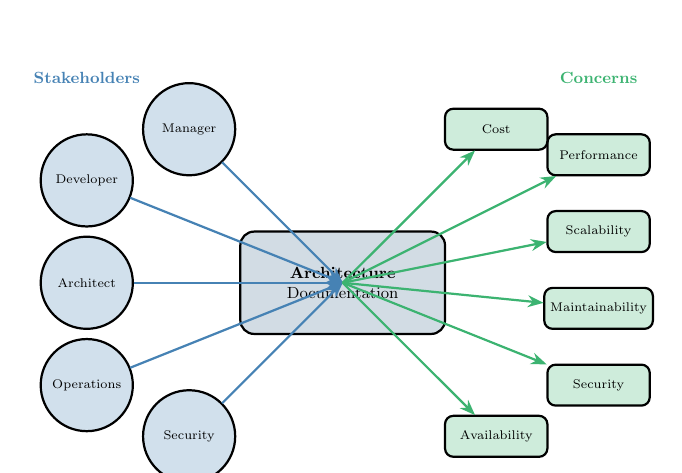
\begin{tikzpicture}[
    scale=0.65,
    transform shape,
    stakeholder/.style={draw, thick, fill=stakeholdercolor!25, circle, minimum size=1.8cm, font=\scriptsize, align=center},
    concern/.style={draw, thick, fill=concerncolor!25, rounded corners=3pt, minimum width=2cm, minimum height=0.8cm, font=\scriptsize, align=center},
    view/.style={draw, thick, fill=viewcolor!25, minimum width=2.5cm, minimum height=1cm, rounded corners=5pt, font=\small, align=center},
    arrow/.style={-{Stealth[length=2mm]}, thick}
]
    % Central Architecture
    \node[view, minimum width=4cm, minimum height=2cm, fill=sectionblue!20] (arch) at (0,0) {\textbf{Architecture}\\Documentation};
    
    % Stakeholders (left)
    \node[stakeholder] (dev) at (-5,2) {Developer};
    \node[stakeholder] (arch) at (-5,0) {Architect};
    \node[stakeholder] (ops) at (-5,-2) {Operations};
    \node[stakeholder] (mgr) at (-3,3) {Manager};
    \node[stakeholder] (sec) at (-3,-3) {Security};
    
    % Concerns (right)
    \node[concern] (perf) at (5,2.5) {Performance};
    \node[concern] (scale) at (5,1) {Scalability};
    \node[concern] (maint) at (5,-0.5) {Maintainability};
    \node[concern] (secu) at (5,-2) {Security};
    \node[concern] (cost) at (3,3) {Cost};
    \node[concern] (avail) at (3,-3) {Availability};
    
    % Connections
    \draw[arrow, stakeholdercolor] (dev) -- (0,0);
    \draw[arrow, stakeholdercolor] (arch) -- (0,0);
    \draw[arrow, stakeholdercolor] (ops) -- (0,0);
    \draw[arrow, stakeholdercolor] (mgr) -- (0,0);
    \draw[arrow, stakeholdercolor] (sec) -- (0,0);
    
    \draw[arrow, concerncolor] (0,0) -- (perf);
    \draw[arrow, concerncolor] (0,0) -- (scale);
    \draw[arrow, concerncolor] (0,0) -- (maint);
    \draw[arrow, concerncolor] (0,0) -- (secu);
    \draw[arrow, concerncolor] (0,0) -- (cost);
    \draw[arrow, concerncolor] (0,0) -- (avail);
    
    % Labels
    \node[font=\small\bfseries, text=stakeholdercolor] at (-5,4) {Stakeholders};
    \node[font=\small\bfseries, text=concerncolor] at (5,4) {Concerns};
\end{tikzpicture}
\end{center}

\newpage
\tableofcontents
\newpage

%==============================================================================
\section{Introduction}
%==============================================================================

\subsection{Purpose of This Guide}

This guide provides a systematic approach to identifying stakeholders and their concerns for software architecture documentation. It serves as both an instructional reference and a practical toolkit for architects creating or reviewing architecture documentation.

\begin{definition}
\textbf{Stakeholder:} An individual, team, organization, or class thereof, having an interest in a system (ISO/IEC/IEEE 42010). Stakeholders include anyone who uses, develops, operates, maintains, sponsors, or is affected by the system or its documentation.
\end{definition}

\begin{definition}
\textbf{Concern:} An interest in a system relevant to one or more of its stakeholders (ISO/IEC/IEEE 42010). Concerns include system qualities, behaviors, constraints, and any other aspect of interest to stakeholders.
\end{definition}

\subsection{Why Stakeholders and Concerns Matter}

Architecture documentation exists to serve stakeholders. Without understanding who will use the documentation and what information they need, architects risk creating documentation that is either incomplete (missing critical information) or bloated (containing unused detail).

\begin{warning}
\textbf{Common Failures from Poor Stakeholder Analysis:}

\textbf{Missing stakeholders:} Security team not consulted; security mechanisms inadequately documented; vulnerabilities discovered late.

\textbf{Overlooked concerns:} Operations team's deployment concerns ignored; documentation lacks deployment view; painful production rollouts.

\textbf{Wrong level of detail:} Executives receive highly technical views; developers receive high-level summaries; neither group served.

\textbf{Undocumented assumptions:} Stakeholder assumptions not captured; implicit requirements violated; costly rework.
\end{warning}

\subsection{Relationship to Architecture Documentation}

Stakeholder and concern analysis drives all aspects of architecture documentation:

\begin{figure}[H]
\centering
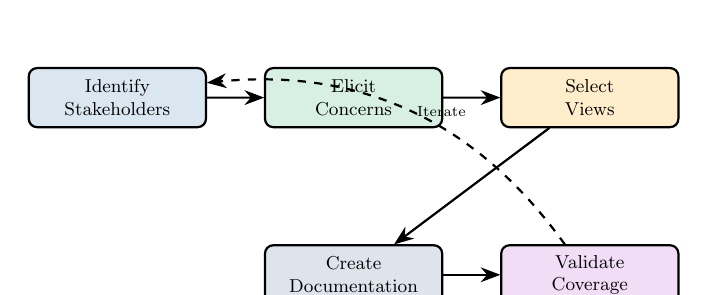
\begin{tikzpicture}[
    scale=0.75,
    transform shape,
    box/.style={draw, thick, rounded corners=3pt, minimum width=3cm, minimum height=1cm, font=\small, align=center},
    arrow/.style={-{Stealth[length=2.5mm]}, thick}
]
    % Process flow
    \node[box, fill=stakeholdercolor!20] (identify) at (0,3) {Identify\\Stakeholders};
    \node[box, fill=concerncolor!20] (elicit) at (4,3) {Elicit\\Concerns};
    \node[box, fill=viewcolor!20] (select) at (8,3) {Select\\Views};
    \node[box, fill=sectionblue!15] (create) at (4,0) {Create\\Documentation};
    \node[box, fill=decisioncolor!20] (validate) at (8,0) {Validate\\Coverage};
    
    % Arrows
    \draw[arrow] (identify) -- (elicit);
    \draw[arrow] (elicit) -- (select);
    \draw[arrow] (select) -- (create);
    \draw[arrow] (create) -- (validate);
    \draw[arrow, dashed] (validate) to[bend right=30] node[right, font=\scriptsize] {Iterate} (identify);
\end{tikzpicture}
\caption{Stakeholder-Driven Documentation Process}
\end{figure}

\subsection{Standards and Frameworks}

This guide aligns with established standards and methodologies:

\begin{itemize}
    \item \textbf{ISO/IEC/IEEE 42010:2011} --- Systems and software engineering---Architecture description; defines stakeholders and concerns as fundamental concepts
    \item \textbf{SEI Views and Beyond} --- Provides stakeholder-driven approach to view selection
    \item \textbf{TOGAF} --- Includes stakeholder management in Architecture Development Method
    \item \textbf{Rozanski \& Woods} --- Software Systems Architecture with stakeholder-concern-viewpoint framework
    \item \textbf{IEEE 1471-2000} --- Predecessor to ISO 42010; established stakeholder-centric approach
\end{itemize}

%==============================================================================
\section{Stakeholder Taxonomy}
%==============================================================================

\subsection{Stakeholder Categories}

Stakeholders can be organized into categories based on their relationship to the system.

\begin{figure}[H]
\centering
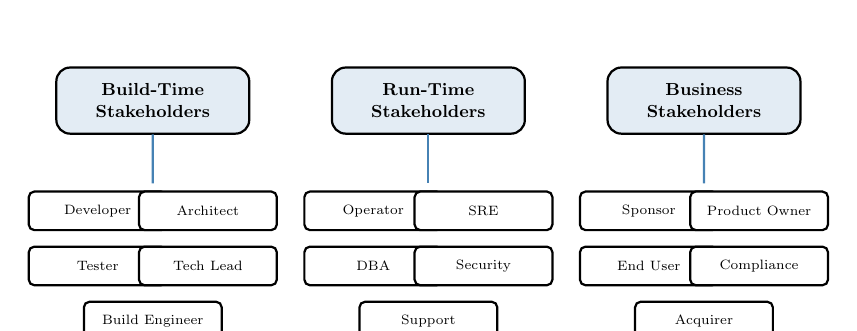
\begin{tikzpicture}[
    scale=0.7,
    transform shape,
    category/.style={draw, thick, fill=stakeholdercolor!15, minimum width=3.5cm, minimum height=1.2cm, rounded corners=5pt, font=\small\bfseries, align=center},
    role/.style={draw, thick, fill=white, minimum width=2.5cm, minimum height=0.7cm, rounded corners=2pt, font=\scriptsize, align=center}
]
    % Categories
    \node[category] (build) at (-5,2) {Build-Time\\Stakeholders};
    \node[category] (runtime) at (0,2) {Run-Time\\Stakeholders};
    \node[category] (business) at (5,2) {Business\\Stakeholders};
    
    % Build-time roles
    \node[role] at (-6,0) {Developer};
    \node[role] at (-4,0) {Architect};
    \node[role] at (-6,-1) {Tester};
    \node[role] at (-4,-1) {Tech Lead};
    \node[role] at (-5,-2) {Build Engineer};
    
    % Runtime roles
    \node[role] at (-1,0) {Operator};
    \node[role] at (1,0) {SRE};
    \node[role] at (-1,-1) {DBA};
    \node[role] at (1,-1) {Security};
    \node[role] at (0,-2) {Support};
    
    % Business roles
    \node[role] at (4,0) {Sponsor};
    \node[role] at (6,0) {Product Owner};
    \node[role] at (4,-1) {End User};
    \node[role] at (6,-1) {Compliance};
    \node[role] at (5,-2) {Acquirer};
    
    % Connections
    \draw[thick, stakeholdercolor] (build) -- (-5,0.5);
    \draw[thick, stakeholdercolor] (runtime) -- (0,0.5);
    \draw[thick, stakeholdercolor] (business) -- (5,0.5);
\end{tikzpicture}
\caption{Stakeholder Categories}
\end{figure}

\subsection{Comprehensive Stakeholder Catalog}

The following catalog provides a reference list of common stakeholders. Not all stakeholders apply to every project; use this as a checklist to ensure no relevant stakeholders are overlooked.

\begin{longtable}{@{}L{2.5cm} L{4cm} L{6cm}@{}}
\caption{Build-Time Stakeholders} \\
\toprule
\textbf{Stakeholder} & \textbf{Role Description} & \textbf{Primary Interests} \\
\midrule
\endfirsthead
\toprule
\textbf{Stakeholder} & \textbf{Role Description} & \textbf{Primary Interests} \\
\midrule
\endhead
\bottomrule
\endlastfoot
Software Architect & Defines system structure and key decisions & Technical coherence; quality attributes; design rationale \\
Developer & Implements system components & Component responsibilities; interfaces; dependencies; coding standards \\
Tech Lead & Leads development team; makes technical decisions & Team boundaries; integration points; technical feasibility \\
QA Engineer & Designs and executes tests & Testability; component boundaries; test environments \\
Build Engineer & Manages build and CI/CD pipelines & Build dependencies; artifact structure; deployment automation \\
Database Admin & Designs and maintains databases & Data models; performance; backup/recovery; migrations \\
UI/UX Designer & Creates user interface designs & User interaction patterns; frontend architecture \\
Technical Writer & Creates documentation & Documentation structure; terminology; audience needs \\
Security Engineer & Ensures security requirements met & Security mechanisms; threat models; compliance \\
Performance Engineer & Optimizes system performance & Performance characteristics; bottlenecks; benchmarks \\
\end{longtable}

\begin{longtable}{@{}L{2.5cm} L{4cm} L{6cm}@{}}
\caption{Run-Time Stakeholders} \\
\toprule
\textbf{Stakeholder} & \textbf{Role Description} & \textbf{Primary Interests} \\
\midrule
\endfirsthead
\toprule
\textbf{Stakeholder} & \textbf{Role Description} & \textbf{Primary Interests} \\
\midrule
\endhead
\bottomrule
\endlastfoot
System Administrator & Deploys and configures systems & Deployment procedures; configuration; administration tools \\
Operator & Monitors and maintains running systems & Operational procedures; monitoring; troubleshooting \\
SRE & Ensures reliability and availability & Reliability patterns; incident response; SLOs \\
Network Engineer & Manages network infrastructure & Network topology; protocols; security zones \\
Help Desk / Support & Provides user support & Error messages; diagnostic procedures; escalation paths \\
End User & Uses the system directly & Functionality; usability; response time \\
System Integrator & Integrates with other systems & APIs; protocols; data formats; integration patterns \\
Data Analyst & Analyzes system data & Data access; reporting capabilities; analytics \\
Auditor & Verifies compliance & Audit trails; access controls; compliance evidence \\
\end{longtable}

\begin{longtable}{@{}L{2.5cm} L{4cm} L{6cm}@{}}
\caption{Business Stakeholders} \\
\toprule
\textbf{Stakeholder} & \textbf{Role Description} & \textbf{Primary Interests} \\
\midrule
\endfirsthead
\toprule
\textbf{Stakeholder} & \textbf{Role Description} & \textbf{Primary Interests} \\
\midrule
\endhead
\bottomrule
\endlastfoot
Project Sponsor & Funds and champions the project & ROI; schedule; budget; risk \\
Product Owner & Defines product requirements & Feature delivery; business value; roadmap \\
Project Manager & Manages project execution & Schedule; resources; dependencies; risks \\
Business Analyst & Translates business needs & Requirements; use cases; business rules \\
Enterprise Architect & Ensures enterprise alignment & Standards compliance; reuse; integration \\
Compliance Officer & Ensures regulatory compliance & Regulations; policies; audit requirements \\
Legal Counsel & Manages legal aspects & Licensing; liability; contracts; IP \\
Procurement & Acquires products and services & Vendor evaluation; contracts; costs \\
Customer & External purchaser/user & Capabilities; quality; support; pricing \\
Partner & External organization with integration & APIs; SLAs; data sharing; security \\
\end{longtable}

\subsection{Stakeholder Identification Process}

\begin{bestpractice}
\textbf{Systematic Stakeholder Identification:}

\begin{enumerate}
    \item \textbf{Start with the catalog:} Review the stakeholder catalog above as a checklist
    
    \item \textbf{Analyze the lifecycle:} Consider who is involved in each phase:
    \begin{itemize}[nosep]
        \item Requirements and design
        \item Development and testing
        \item Deployment and operations
        \item Maintenance and evolution
        \item Retirement and replacement
    \end{itemize}
    
    \item \textbf{Follow the money:} Identify who funds, purchases, or benefits financially
    
    \item \textbf{Follow the data:} Identify who creates, uses, or is affected by system data
    
    \item \textbf{Consider external entities:} Regulators, partners, competitors, public
    
    \item \textbf{Ask stakeholders:} Each identified stakeholder may know of others
    
    \item \textbf{Review organizational charts:} Identify affected departments and roles
    
    \item \textbf{Document and validate:} Create stakeholder list; validate with project leadership
\end{enumerate}
\end{bestpractice}

\subsection{Stakeholder Prioritization}

Not all stakeholders have equal influence or interest. Prioritization helps focus effort on the most important stakeholders.

\begin{figure}[H]
\centering
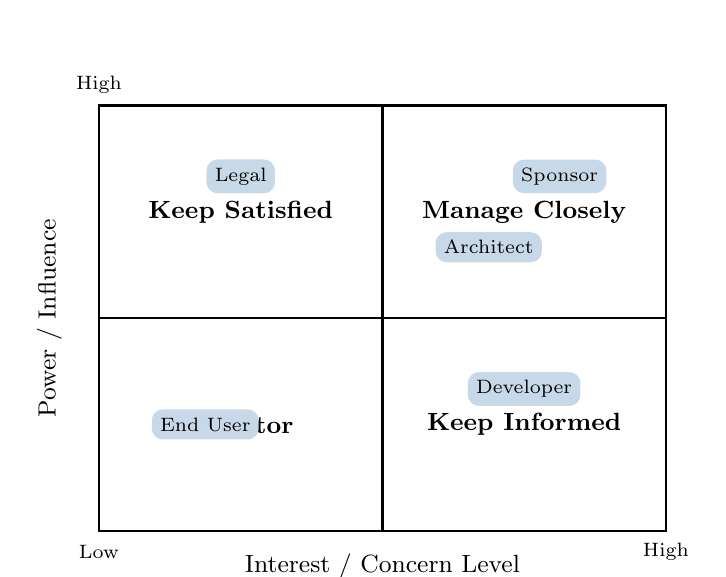
\begin{tikzpicture}[
    scale=0.9
]
    % Grid
    \draw[thick] (0,0) rectangle (8,6);
    \draw[thick] (4,0) -- (4,6);
    \draw[thick] (0,3) -- (8,3);
    
    % Quadrant labels
    \node[font=\small\bfseries] at (2,4.5) {Keep Satisfied};
    \node[font=\small\bfseries] at (6,4.5) {Manage Closely};
    \node[font=\small\bfseries] at (2,1.5) {Monitor};
    \node[font=\small\bfseries] at (6,1.5) {Keep Informed};
    
    % Axis labels
    \node[font=\small, rotate=90] at (-0.7,3) {Power / Influence};
    \node[font=\small] at (4,-0.5) {Interest / Concern Level};
    
    \node[font=\scriptsize] at (0,6.3) {High};
    \node[font=\scriptsize] at (0,-0.3) {Low};
    \node[font=\scriptsize] at (8,-0.3) {High};
    
    % Example stakeholders
    \node[fill=stakeholdercolor!30, rounded corners, font=\scriptsize, inner sep=3pt] at (6.5,5) {Sponsor};
    \node[fill=stakeholdercolor!30, rounded corners, font=\scriptsize, inner sep=3pt] at (5.5,4) {Architect};
    \node[fill=stakeholdercolor!30, rounded corners, font=\scriptsize, inner sep=3pt] at (6,2) {Developer};
    \node[fill=stakeholdercolor!30, rounded corners, font=\scriptsize, inner sep=3pt] at (2,5) {Legal};
    \node[fill=stakeholdercolor!30, rounded corners, font=\scriptsize, inner sep=3pt] at (1.5,1.5) {End User};
\end{tikzpicture}
\caption{Stakeholder Power/Interest Matrix}
\end{figure}

\begin{longtable}{@{}L{3cm} L{4.5cm} L{5cm}@{}}
\caption{Stakeholder Engagement Strategies} \\
\toprule
\textbf{Quadrant} & \textbf{Characteristics} & \textbf{Engagement Strategy} \\
\midrule
\endfirsthead
\bottomrule
\endlastfoot
Manage Closely & High power, high interest & Active engagement; regular consultation; address concerns promptly \\
Keep Satisfied & High power, low interest & Keep informed of major decisions; don't overwhelm with detail \\
Keep Informed & Low power, high interest & Regular updates; address concerns; leverage their knowledge \\
Monitor & Low power, low interest & Minimal effort; periodic check-ins; monitor for changing interest \\
\end{longtable}

%==============================================================================
\section{Concern Taxonomy}
%==============================================================================

\subsection{What is a Concern?}

\begin{definition}
A \textbf{concern} is any interest in a system that is relevant to one or more stakeholders. Concerns encompass system qualities (performance, security), system behaviors (functionality), constraints (technology mandates, regulations), and any other aspect that stakeholders care about.
\end{definition}

Concerns drive architecture documentation by determining what information must be captured and communicated.

\subsection{Concern Categories}

\begin{figure}[H]
\centering
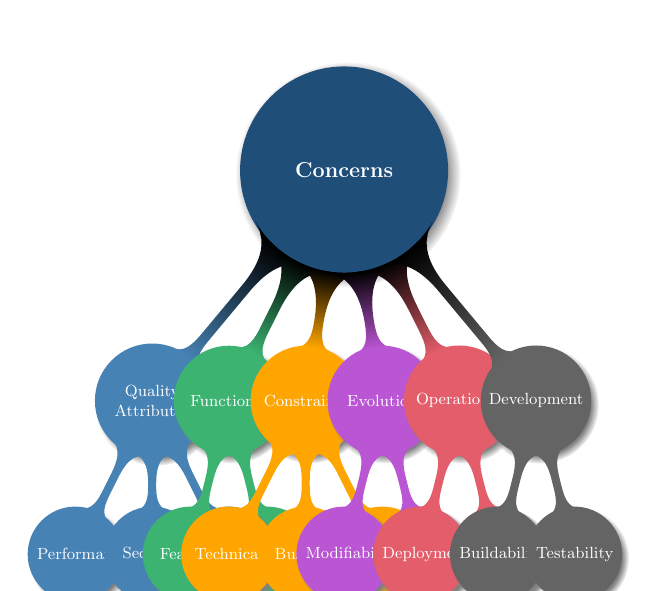
\begin{tikzpicture}[
    scale=0.65,
    transform shape,
    mindmap,
    every node/.style={concept, circular drop shadow, minimum size=18mm, text=white, font=\small},
    root concept/.append style={concept color=sectionblue, font=\large\bfseries},
    level 1 concept/.append style={level distance=4.5cm, sibling angle=60},
    level 2 concept/.append style={level distance=3cm, sibling angle=45, font=\scriptsize}
]
    \node[root concept] {Concerns}
        child[concept color=stakeholdercolor] { node {Quality\\Attributes}
            child { node {Performance} }
            child { node {Security} }
            child { node {Availability} }
        }
        child[concept color=concerncolor] { node {Functional}
            child { node {Features} }
            child { node {Behavior} }
        }
        child[concept color=viewcolor] { node {Constraints}
            child { node {Technical} }
            child { node {Business} }
            child { node {Regulatory} }
        }
        child[concept color=decisioncolor] { node {Evolution}
            child { node {Modifiability} }
            child { node {Extensibility} }
        }
        child[concept color=warningred!80] { node {Operational}
            child { node {Deployment} }
            child { node {Monitoring} }
        }
        child[concept color=flowcolor] { node {Development}
            child { node {Buildability} }
            child { node {Testability} }
        };
\end{tikzpicture}
\caption{Concern Category Mind Map}
\end{figure}

\subsection{Comprehensive Concern Catalog}

\subsubsection{Quality Attribute Concerns}

Quality attributes (also called non-functional requirements) are often the most architecturally significant concerns.

\begin{longtable}{@{}L{2.5cm} L{5cm} L{5cm}@{}}
\caption{Quality Attribute Concerns} \\
\toprule
\textbf{Quality Attribute} & \textbf{Definition} & \textbf{Typical Stakeholders} \\
\midrule
\endfirsthead
\toprule
\textbf{Quality Attribute} & \textbf{Definition} & \textbf{Typical Stakeholders} \\
\midrule
\endhead
\bottomrule
\endlastfoot
Performance & Response time, throughput, resource utilization & End users; Operations; Performance engineers \\
Scalability & Ability to handle increased load & Architects; Operations; Capacity planners \\
Availability & System uptime; fault tolerance & End users; Operations; SREs; Business \\
Reliability & Consistency of correct behavior over time & End users; QA; Operations \\
Security & Protection against threats; confidentiality; integrity & Security team; Compliance; End users \\
Maintain\-ability & Ease of modification and correction & Developers; Architects; Maintainers \\
Modifiability & Ability to make changes at reasonable cost & Architects; Developers; Product owners \\
Testability & Ease of testing and verification & QA engineers; Developers \\
Usability & Ease of use; user experience & End users; UX designers; Product owners \\
Inter\-operability & Ability to work with other systems & System integrators; Partners; Architects \\
Portability & Ability to run in different environments & Operations; Architects; Enterprise architects \\
Deployability & Ease of deployment and updates & Operations; DevOps; Release managers \\
Monitorability & Ability to observe system behavior & Operations; SREs; Support \\
Recoverability & Ability to recover from failures & Operations; Business continuity; DBAs \\
Cost & Development and operational expenses & Sponsors; Finance; Management \\
\end{longtable}

\subsubsection{Functional Concerns}

\begin{longtable}{@{}L{3cm} L{5cm} L{4.5cm}@{}}
\caption{Functional Concerns} \\
\toprule
\textbf{Concern} & \textbf{Description} & \textbf{Typical Stakeholders} \\
\midrule
\endfirsthead
\bottomrule
\endlastfoot
Feature completeness & All required features implemented & Product owners; Business analysts \\
Data integrity & Data remains accurate and consistent & DBAs; Data engineers; Compliance \\
Business rules & Correct implementation of business logic & Business analysts; Domain experts \\
User workflows & Support for user tasks and processes & End users; UX designers \\
Integration & Connectivity with external systems & System integrators; Partners \\
Reporting & Generation of required reports & Business users; Data analysts \\
\end{longtable}

\subsubsection{Constraint Concerns}

\begin{longtable}{@{}L{3cm} L{5cm} L{4.5cm}@{}}
\caption{Constraint Concerns} \\
\toprule
\textbf{Concern} & \textbf{Description} & \textbf{Typical Stakeholders} \\
\midrule
\endfirsthead
\bottomrule
\endlastfoot
Technology mandates & Required technologies or platforms & Enterprise architects; IT governance \\
Standards compliance & Adherence to technical standards & Architects; Compliance \\
Regulatory compliance & Meeting legal/regulatory requirements & Compliance; Legal; Auditors \\
Budget constraints & Development and operational budget limits & Sponsors; Finance; Management \\
Schedule constraints & Delivery timeline requirements & Project managers; Sponsors \\
Resource constraints & Available people and skills & Project managers; HR \\
Legacy integration & Compatibility with existing systems & Enterprise architects; Operations \\
Vendor relationships & Use of specific vendors or products & Procurement; Enterprise architects \\
\end{longtable}

\subsubsection{Development Concerns}

\begin{longtable}{@{}L{3cm} L{5cm} L{4.5cm}@{}}
\caption{Development Concerns} \\
\toprule
\textbf{Concern} & \textbf{Description} & \textbf{Typical Stakeholders} \\
\midrule
\endfirsthead
\bottomrule
\endlastfoot
Code organization & How code is structured and organized & Developers; Tech leads; Architects \\
Build process & How system is compiled and packaged & Build engineers; DevOps \\
Development environment & Tools and setup for development & Developers; Tech leads \\
Team structure & How teams are organized around code & Management; Tech leads \\
Coding standards & Conventions and style guidelines & Developers; Tech leads \\
Dependency management & External library and service dependencies & Developers; Security; Architects \\
Version control & Source code management approach & Developers; Build engineers \\
\end{longtable}

\subsubsection{Operational Concerns}

\begin{longtable}{@{}L{3cm} L{5cm} L{4.5cm}@{}}
\caption{Operational Concerns} \\
\toprule
\textbf{Concern} & \textbf{Description} & \textbf{Typical Stakeholders} \\
\midrule
\endfirsthead
\bottomrule
\endlastfoot
Deployment & How system is deployed to production & Operations; DevOps; SREs \\
Configuration & How system is configured per environment & Operations; Developers \\
Monitoring & How system behavior is observed & Operations; SREs \\
Logging & What is logged and how & Operations; Security; Support \\
Alerting & How problems are detected and reported & Operations; SREs \\
Backup/Recovery & Data protection and restoration & DBAs; Operations; Business continuity \\
Disaster recovery & Recovery from major failures & Business continuity; Operations \\
Capacity planning & Planning for growth & Capacity planners; Operations \\
Incident response & Handling production issues & SREs; Support; Operations \\
\end{longtable}

%==============================================================================
\section{Concern Elicitation}
%==============================================================================

\subsection{Elicitation Techniques}

Multiple techniques should be used to ensure comprehensive concern identification.

\begin{longtable}{@{}L{3cm} L{4.5cm} L{5cm}@{}}
\caption{Concern Elicitation Techniques} \\
\toprule
\textbf{Technique} & \textbf{Description} & \textbf{When to Use} \\
\midrule
\endfirsthead
\toprule
\textbf{Technique} & \textbf{Description} & \textbf{When to Use} \\
\midrule
\endhead
\bottomrule
\endlastfoot
Stakeholder Interviews & One-on-one discussions with stakeholders & Key stakeholders; sensitive concerns; deep exploration \\
Workshops & Facilitated group sessions & Multiple stakeholders; cross-cutting concerns; consensus building \\
Questionnaires & Written questions distributed to stakeholders & Large stakeholder groups; remote stakeholders; initial gathering \\
Document Analysis & Review of existing documentation & Legacy systems; regulatory requirements; organizational standards \\
Catalog Review & Walk through concern catalog with stakeholders & Ensuring completeness; prompting discussion \\
Scenario Analysis & Explore system behavior in specific situations & Quality attributes; edge cases; failure modes \\
Prototype Review & Stakeholders review early system versions & User-facing concerns; usability; workflow validation \\
Quality Attribute Workshop (QAW) & SEI method for eliciting quality requirements & Quality attribute prioritization; scenario development \\
\end{longtable}

\subsection{Interview Guidelines}

\begin{stakeholderbox}[Stakeholder Interview Template]

\textbf{Pre-Interview Preparation}
\begin{itemize}[nosep]
    \item Review stakeholder's role and organizational context
    \item Identify likely concerns based on role
    \item Prepare role-specific questions
    \item Schedule 60-90 minutes
\end{itemize}

\vspace{0.3cm}
\textbf{Opening (5 minutes)}
\begin{itemize}[nosep]
    \item Introduce purpose: understanding their perspective on the system
    \item Explain how information will be used
    \item Confirm time available
\end{itemize}

\vspace{0.3cm}
\textbf{Core Questions (45-60 minutes)}
\begin{enumerate}[nosep]
    \item Describe your role and how you interact with this system
    \item What does success look like for you with this system?
    \item What are your biggest concerns or worries about the system?
    \item What information about the system do you need to do your job?
    \item What problems have you experienced with similar systems?
    \item What quality attributes matter most to you? (performance, security, etc.)
    \item Are there constraints or regulations that affect your work?
    \item Who else should we talk to about concerns like yours?
    \item What questions do you have that the architecture documentation should answer?
\end{enumerate}

\vspace{0.3cm}
\textbf{Closing (5-10 minutes)}
\begin{itemize}[nosep]
    \item Summarize key concerns captured
    \item Ask if anything was missed
    \item Explain next steps and follow-up
    \item Thank stakeholder for their time
\end{itemize}

\vspace{0.3cm}
\textbf{Post-Interview}
\begin{itemize}[nosep]
    \item Document concerns within 24 hours
    \item Categorize concerns using taxonomy
    \item Identify concerns requiring follow-up
    \item Send summary to stakeholder for validation
\end{itemize}
\end{stakeholderbox}

\subsection{Quality Attribute Workshop (QAW)}

The SEI's Quality Attribute Workshop is a structured method for eliciting and prioritizing quality attribute concerns.

\begin{figure}[H]
\centering
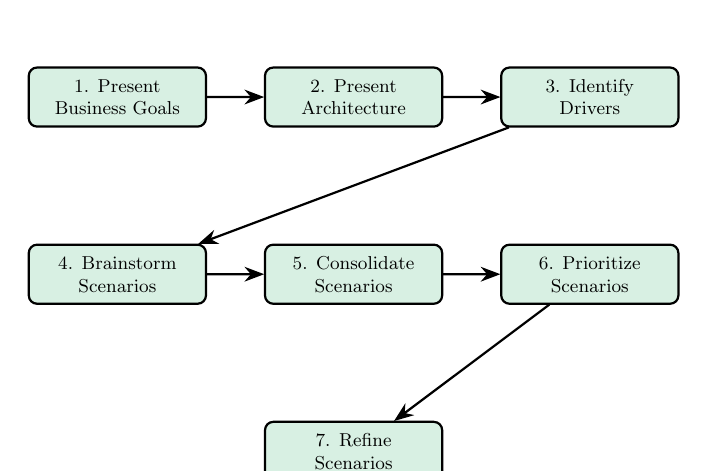
\begin{tikzpicture}[
    scale=0.75,
    transform shape,
    processstep/.style={draw, thick, fill=concerncolor!20, minimum width=3cm, minimum height=1cm, rounded corners=3pt, font=\small, align=center},
    arrow/.style={-{Stealth[length=2.5mm]}, thick}
]
    % Steps
    \node[processstep] (s1) at (0,4) {1. Present\\Business Goals};
    \node[processstep] (s2) at (4,4) {2. Present\\Architecture};
    \node[processstep] (s3) at (8,4) {3. Identify\\Drivers};
    \node[processstep] (s4) at (0,1) {4. Brainstorm\\Scenarios};
    \node[processstep] (s5) at (4,1) {5. Consolidate\\Scenarios};
    \node[processstep] (s6) at (8,1) {6. Prioritize\\Scenarios};
    \node[processstep] (s7) at (4,-2) {7. Refine\\Scenarios};
    
    % Arrows
    \draw[arrow] (s1) -- (s2);
    \draw[arrow] (s2) -- (s3);
    \draw[arrow] (s3) -- (s4);
    \draw[arrow] (s4) -- (s5);
    \draw[arrow] (s5) -- (s6);
    \draw[arrow] (s6) -- (s7);
\end{tikzpicture}
\caption{Quality Attribute Workshop Process}
\end{figure}

\textbf{QAW Outputs:}
\begin{itemize}
    \item Prioritized list of quality attribute scenarios
    \item Business goals and their architectural implications
    \item Architectural drivers (most important quality concerns)
    \item Stakeholder consensus on priorities
\end{itemize}

%==============================================================================
\section{Mapping Concerns to Views}
%==============================================================================

\subsection{The Mapping Challenge}

Once concerns are identified, they must be mapped to architectural views that address them. This mapping ensures that:
\begin{itemize}
    \item Every concern is addressed by at least one view
    \item Views are created for the most important concerns
    \item Stakeholders know where to find information about their concerns
\end{itemize}

\subsection{Concern-View Mapping Matrix}

\begin{longtable}{@{}L{2.5cm} C{1.3cm} C{1.3cm} C{1.3cm} C{1.3cm} C{1.3cm} C{1.3cm}@{}}
\caption{Concern-View Mapping Matrix} \\
\toprule
\textbf{Concern} & \textbf{Module} & \textbf{C\&C} & \textbf{Deploy} & \textbf{Data} & \textbf{Context} & \textbf{Rationale} \\
\midrule
\endfirsthead
\toprule
\textbf{Concern} & \textbf{Module} & \textbf{C\&C} & \textbf{Deploy} & \textbf{Data} & \textbf{Context} & \textbf{Rationale} \\
\midrule
\endhead
\bottomrule
\endlastfoot
Performance & $\circ$ & $\bullet$ & $\bullet$ & $\circ$ & & $\circ$ \\
Scalability & & $\bullet$ & $\bullet$ & & & $\circ$ \\
Availability & & $\bullet$ & $\bullet$ & & & $\circ$ \\
Security & $\circ$ & $\bullet$ & $\bullet$ & $\bullet$ & $\circ$ & $\bullet$ \\
Maintain\-ability & $\bullet$ & & & & & $\circ$ \\
Modifiability & $\bullet$ & $\circ$ & & & & $\bullet$ \\
Testability & $\bullet$ & $\circ$ & & & & \\
Deployability & & & $\bullet$ & & & \\
Code organization & $\bullet$ & & & & & \\
Data integrity & & & & $\bullet$ & & \\
Integration & & $\bullet$ & & & $\bullet$ & \\
Cost & & & $\bullet$ & & & $\bullet$ \\
\multicolumn{7}{l}{\scriptsize $\bullet$ = Primary view \quad $\circ$ = Secondary view} \\
\end{longtable}

\subsection{Stakeholder-View Navigation Guide}

\begin{longtable}{@{}L{2.5cm} L{4cm} L{6cm}@{}}
\caption{Stakeholder-View Navigation} \\
\toprule
\textbf{Stakeholder} & \textbf{Primary Views} & \textbf{Key Information Sought} \\
\midrule
\endfirsthead
\toprule
\textbf{Stakeholder} & \textbf{Primary Views} & \textbf{Key Information Sought} \\
\midrule
\endhead
\bottomrule
\endlastfoot
Developer & Module; C\&C & Component responsibilities; interfaces; dependencies \\
Architect & All views & Design decisions; trade-offs; quality attributes \\
Tech Lead & Module; C\&C & Team boundaries; integration points \\
QA Engineer & Module; C\&C & Testable components; interfaces; scenarios \\
Operations & Deployment; C\&C & Infrastructure; monitoring; procedures \\
SRE & Deployment; C\&C & Reliability patterns; failure modes; recovery \\
Security & C\&C; Deployment; Data & Security mechanisms; trust boundaries \\
DBA & Data; Deployment & Data models; storage; backup \\
Product Owner & Context; Rationale & Capabilities; decisions; roadmap implications \\
Sponsor & Context; Rationale & Business value; risks; costs \\
\end{longtable}

%==============================================================================
\section{Review Question Sets}
%==============================================================================

This section provides structured question sets for reviewing stakeholder and concern coverage in architecture documentation.

\subsection{Question Set Overview}

\begin{keypoint}
\textbf{Purpose:} These question sets verify that the architect has identified appropriate stakeholders and concerns and that these are adequately represented in the architecture description. They enable both self-review by architects and formal reviews by stakeholder groups.
\end{keypoint}

\subsection{Questions for All Stakeholders}

\begin{questionbox}[Stakeholder Self-Assessment Questions]

\textbf{Instructions:} Each stakeholder should answer these questions independently, then discuss findings in a review session.

\vspace{0.3cm}
\textbf{Role and Concern Identification}
\begin{enumerate}
    \item State your stakeholder role(s). What decisions do you make or actions do you take that depend on the architecture?
    
    \item List all concerns you have that pertain to the architecture. For each concern:
    \begin{itemize}[nosep]
        \item Why does this concern matter to you?
        \item What would be the impact if this concern were not addressed?
        \item How would you measure whether the concern is satisfied?
    \end{itemize}
    
    \item Prioritize your concerns (High/Medium/Low) based on their impact on your ability to perform your role.
\end{enumerate}

\vspace{0.3cm}
\textbf{Coverage Assessment}
\begin{enumerate}[resume]
    \item Find and record all places in the architecture description where your stakeholder role is explicitly mentioned or addressed.
    
    \item For each of your concerns, find and record where in the documentation that concern is:
    \begin{itemize}[nosep]
        \item Listed or acknowledged
        \item Actually addressed with architectural content
    \end{itemize}
    
    \item Rate how well each concern is addressed:
    \begin{itemize}[nosep]
        \item \textbf{Well addressed:} Clear, complete information enabling decisions
        \item \textbf{Partially addressed:} Some information, but gaps remain
        \item \textbf{Acknowledged only:} Listed but not substantively addressed
        \item \textbf{Not addressed:} No mention or coverage
    \end{itemize}
    
    \item For concerns not well addressed, describe:
    \begin{itemize}[nosep]
        \item What specific information is missing?
        \item What decisions can you not make without this information?
        \item What is the impact of this gap on project success?
    \end{itemize}
\end{enumerate}

\vspace{0.3cm}
\textbf{Gap Identification}
\begin{enumerate}[resume]
    \item Identify any stakeholder roles you are aware of that are not represented in the architect's stakeholder list. For each:
    \begin{itemize}[nosep]
        \item What is the role?
        \item Why should they be included?
        \item What concerns would they likely have?
    \end{itemize}
    
    \item Identify any concerns that should be in the documentation but are not, including:
    \begin{itemize}[nosep]
        \item Concerns for missing stakeholders
        \item Additional concerns for your own role
        \item Cross-cutting concerns affecting multiple stakeholders
    \end{itemize}
    
    \item For each missing concern, assess:
    \begin{itemize}[nosep]
        \item Criticality (High/Medium/Low)
        \item Impact if not addressed
        \item Suggested approach for addressing
    \end{itemize}
\end{enumerate}

\vspace{0.3cm}
\textbf{Usability Assessment}
\begin{enumerate}[resume]
    \item Rate the ease of finding information relevant to your concerns:
    \begin{itemize}[nosep]
        \item Easy: Intuitive navigation; information where expected
        \item Moderate: Required some searching; eventually found
        \item Difficult: Significant effort to locate; scattered information
        \item Unable: Could not find needed information
    \end{itemize}
    
    \item Provide suggestions for improving documentation organization or navigation for stakeholders in your role.
\end{enumerate}
\end{questionbox}

\subsection{Questions for the Architect}

\begin{questionbox}[Architect Self-Assessment Questions]

\textbf{Stakeholder Identification Process}
\begin{enumerate}
    \item Describe the process you used to identify stakeholders:
    \begin{itemize}[nosep]
        \item What sources did you consult? (org charts, project docs, interviews)
        \item What techniques did you use? (workshops, interviews, checklists)
        \item How did you validate completeness?
    \end{itemize}
    
    \item For each stakeholder category (build-time, run-time, business), explain why specific roles were included or excluded.
    
    \item How did you prioritize stakeholders for documentation focus?
\end{enumerate}

\vspace{0.3cm}
\textbf{Concern Elicitation Process}
\begin{enumerate}[resume]
    \item Describe how you elicited concerns from stakeholders:
    \begin{itemize}[nosep]
        \item Which stakeholders did you interview or consult?
        \item What elicitation techniques did you use?
        \item How did you ensure concerns were accurately captured?
    \end{itemize}
    
    \item How did you prioritize concerns for documentation focus?
    
    \item For quality attribute concerns, describe how you developed quality attribute scenarios or requirements.
\end{enumerate}

\vspace{0.3cm}
\textbf{Coverage Demonstration}
\begin{enumerate}[resume]
    \item Show where in the documentation each identified stakeholder role is addressed.
    
    \item For each documented concern, show:
    \begin{itemize}[nosep]
        \item Which view(s) address the concern
        \item How the concern is satisfied by the architecture
        \item Any trade-offs made affecting the concern
    \end{itemize}
    
    \item Demonstrate that every concern traces to at least one stakeholder.
    
    \item Demonstrate that every view traces to at least one concern.
\end{enumerate}

\vspace{0.3cm}
\textbf{Framework Alignment}
\begin{enumerate}[resume]
    \item If using an architectural framework (TOGAF, ISO 42010, etc.):
    \begin{itemize}[nosep]
        \item Show where framework-required stakeholders are addressed
        \item Show where framework-required concerns are addressed
        \item Explain any deviations from framework guidance
    \end{itemize}
\end{enumerate}
\end{questionbox}

\subsection{Review Session Guidelines}

\begin{template}
\textbf{Stakeholder Review Session Agenda}

\vspace{0.3cm}
\textbf{Pre-Session (1-2 weeks before)}
\begin{itemize}[nosep]
    \item Distribute architecture documentation to all reviewers
    \item Distribute question sets with response templates
    \item Request completed responses 2 days before session
    \item Compile and analyze responses; identify themes
\end{itemize}

\vspace{0.3cm}
\textbf{Session Agenda (Half-day workshop)}

\textbf{1. Opening (15 minutes)}
\begin{itemize}[nosep]
    \item Welcome and introductions
    \item Review session objectives and ground rules
    \item Overview of architecture documentation structure
\end{itemize}

\textbf{2. Stakeholder Coverage Review (45 minutes)}
\begin{itemize}[nosep]
    \item Present compiled stakeholder coverage findings
    \item Discuss missing or underrepresented stakeholders
    \item Reach consensus on stakeholder list completeness
\end{itemize}

\textbf{3. Concern Coverage Review (90 minutes)}
\begin{itemize}[nosep]
    \item Present compiled concern coverage findings
    \item Walk through each concern category
    \item Identify gaps and inadequately addressed concerns
    \item Prioritize gaps by impact
\end{itemize}

\textbf{4. Architect Response (30 minutes)}
\begin{itemize}[nosep]
    \item Architect responds to findings
    \item Clarifications and additional context
    \item Identify quick fixes vs. significant updates
\end{itemize}

\textbf{5. Action Planning (30 minutes)}
\begin{itemize}[nosep]
    \item Document required changes
    \item Assign owners and deadlines
    \item Schedule follow-up review if needed
\end{itemize}

\textbf{6. Closing (15 minutes)}
\begin{itemize}[nosep]
    \item Summarize decisions and actions
    \item Gather feedback on review process
    \item Thank participants
\end{itemize}
\end{template}

%==============================================================================
\section{Coverage Assessment}
%==============================================================================

\subsection{Stakeholder Coverage Matrix}

\begin{longtable}{@{}L{2.5cm} C{1.5cm} C{1.5cm} C{1.5cm} C{1.5cm} C{2.5cm}@{}}
\caption{Stakeholder Coverage Assessment Template} \\
\toprule
\textbf{Stakeholder} & \textbf{Listed} & \textbf{Concerns Identified} & \textbf{Views Address} & \textbf{Coverage} & \textbf{Gaps} \\
\midrule
\endfirsthead
\toprule
\textbf{Stakeholder} & \textbf{Listed} & \textbf{Concerns Identified} & \textbf{Views Address} & \textbf{Coverage} & \textbf{Gaps} \\
\midrule
\endhead
\bottomrule
\endlastfoot
Developer & \checkmark & \checkmark & Module, C\&C & Full & -- \\
Architect & \checkmark & \checkmark & All & Full & -- \\
Operations & \checkmark & \checkmark & Deploy, C\&C & Partial & Runbooks missing \\
Security & \checkmark & \checkmark & Security View & Full & -- \\
Product Owner & \checkmark & Partial & Context & Partial & Roadmap impact \\
DBA & -- & -- & -- & None & Not consulted \\
\multicolumn{6}{l}{\scriptsize Coverage: Full = All concerns addressed; Partial = Some gaps; None = Not covered} \\
\end{longtable}

\subsection{Concern Traceability Matrix}

\begin{longtable}{@{}L{2.5cm} L{2.5cm} L{2.5cm} C{1.5cm} L{3cm}@{}}
\caption{Concern Traceability Matrix} \\
\toprule
\textbf{Concern} & \textbf{Stakeholders} & \textbf{Addressed In} & \textbf{Priority} & \textbf{Status} \\
\midrule
\endfirsthead
\toprule
\textbf{Concern} & \textbf{Stakeholders} & \textbf{Addressed In} & \textbf{Priority} & \textbf{Status} \\
\midrule
\endhead
\bottomrule
\endlastfoot
Performance & Users, Ops, Perf Eng & C\&C View, Deploy View & High & Addressed \\
Security & Security, Compliance & Security View, Rationale & High & Addressed \\
Scalability & Architect, Ops & C\&C View, Deploy View & High & Addressed \\
Maintain\-ability & Developer, Tech Lead & Module View & Medium & Addressed \\
Testability & QA, Developer & Module View & Medium & Partial \\
Deployability & Ops, DevOps & Deploy View & Medium & Addressed \\
Cost & Sponsor, Finance & Rationale & High & Partial \\
Data migration & DBA, Ops & -- & Medium & Not addressed \\
\end{longtable}

\subsection{Gap Analysis Template}

\begin{template}
\textbf{Documentation Gap Report}

\vspace{0.3cm}
\textbf{Gap ID:} GAP-001

\textbf{Type:} Missing Stakeholder / Missing Concern / Inadequate Coverage

\textbf{Description:} [Clear description of what is missing or inadequate]

\textbf{Affected Stakeholders:} [Who is impacted by this gap]

\textbf{Impact Assessment:}
\begin{itemize}[nosep]
    \item \textbf{Severity:} High / Medium / Low
    \item \textbf{Project Impact:} [How this affects project success]
    \item \textbf{Decision Impact:} [What decisions cannot be made]
\end{itemize}

\textbf{Recommended Resolution:}
\begin{itemize}[nosep]
    \item \textbf{Action:} [What should be done]
    \item \textbf{Owner:} [Who is responsible]
    \item \textbf{Effort:} [Estimated effort to resolve]
    \item \textbf{Deadline:} [When it should be completed]
\end{itemize}

\textbf{Status:} Open / In Progress / Resolved / Deferred

\textbf{Resolution Notes:} [How the gap was addressed]
\end{template}

%==============================================================================
\section{Governance and Maintenance}
%==============================================================================

\subsection{Stakeholder Registry}

Maintain a living registry of stakeholders that evolves with the project.

\begin{longtable}{@{}L{2cm} L{2.5cm} L{2cm} L{2cm} L{2cm} L{2cm}@{}}
\caption{Stakeholder Registry Template} \\
\toprule
\textbf{Name} & \textbf{Role} & \textbf{Category} & \textbf{Priority} & \textbf{Contact} & \textbf{Status} \\
\midrule
\endfirsthead
\bottomrule
\endlastfoot
J. Smith & Lead Developer & Build-time & High & jsmith@ & Active \\
A. Jones & SRE Lead & Run-time & High & ajones@ & Active \\
B. Wilson & Product Owner & Business & High & bwilson@ & Active \\
C. Brown & Security Arch & Build-time & Medium & cbrown@ & Active \\
D. Lee & Project Sponsor & Business & High & dlee@ & Active \\
\end{longtable}

\subsection{Review Cadence}

\begin{longtable}{@{}L{3cm} L{4cm} L{5.5cm}@{}}
\caption{Stakeholder Review Cadence} \\
\toprule
\textbf{Review Type} & \textbf{Frequency} & \textbf{Purpose} \\
\midrule
\endfirsthead
\bottomrule
\endlastfoot
Stakeholder List Review & Quarterly & Verify stakeholder list current; add/remove as needed \\
Concern Coverage Review & Per major release & Verify all concerns still addressed \\
New Stakeholder Onboarding & As needed & Validate documentation meets new stakeholder needs \\
Full Documentation Review & Annually & Comprehensive review of all coverage \\
\end{longtable}

\subsection{Change Management}

\begin{bestpractice}
\textbf{When to Update Stakeholder/Concern Analysis:}

\begin{itemize}
    \item New stakeholder roles identified or organizational changes occur
    \item New concerns emerge from project experience
    \item Regulatory or compliance requirements change
    \item Technology changes introduce new concerns
    \item Post-incident reviews reveal documentation gaps
    \item Stakeholder feedback indicates unmet needs
    \item Architecture undergoes significant changes
\end{itemize}
\end{bestpractice}

%==============================================================================
\section{Appendix A: Stakeholder Interview Questions by Role}
%==============================================================================

\subsection{Developer Interview Questions}

\begin{enumerate}
    \item What components are you responsible for developing?
    \item What information do you need about other components to do your work?
    \item What development standards or patterns should the architecture enforce?
    \item What are your concerns about testability of the system?
    \item What dependencies cause you the most problems?
    \item What would make the codebase easier to work with?
\end{enumerate}

\subsection{Operations Interview Questions}

\begin{enumerate}
    \item What systems will you be responsible for operating?
    \item What deployment procedures do you need documented?
    \item What monitoring and alerting capabilities do you require?
    \item What are your concerns about system reliability?
    \item What backup and recovery procedures do you need?
    \item What capacity planning information do you require?
\end{enumerate}

\subsection{Security Interview Questions}

\begin{enumerate}
    \item What security standards must the system comply with?
    \item What are the most critical assets to protect?
    \item What threat vectors concern you most?
    \item What security controls do you expect to see documented?
    \item What audit and compliance requirements exist?
    \item What security testing will be required?
\end{enumerate}

\subsection{Business Stakeholder Interview Questions}

\begin{enumerate}
    \item What business goals does this system support?
    \item What is the expected return on investment?
    \item What are the critical success factors?
    \item What risks concern you most?
    \item What schedule or budget constraints exist?
    \item How will success be measured?
\end{enumerate}

%==============================================================================
\section{Appendix B: Review Checklist}
%==============================================================================

\subsection{Stakeholder Coverage Checklist}

\begin{itemize}[leftmargin=2cm]
    \item[$\square$] All stakeholder categories considered (build-time, run-time, business)
    \item[$\square$] Key stakeholders identified by name and role
    \item[$\square$] Stakeholder prioritization documented
    \item[$\square$] Each stakeholder's concerns explicitly listed
    \item[$\square$] Stakeholders validated the concern list
    \item[$\square$] Missing stakeholders identified and addressed
    \item[$\square$] Stakeholder contact information maintained
\end{itemize}

\subsection{Concern Coverage Checklist}

\begin{itemize}[leftmargin=2cm]
    \item[$\square$] All concern categories considered (quality, functional, constraint, etc.)
    \item[$\square$] Concerns prioritized by importance
    \item[$\square$] Each concern traced to stakeholders
    \item[$\square$] Each concern mapped to architectural view(s)
    \item[$\square$] Quality attribute scenarios developed for key concerns
    \item[$\square$] Trade-offs between concerns documented
    \item[$\square$] Missing concerns identified and addressed
\end{itemize}

\subsection{Documentation Usability Checklist}

\begin{itemize}[leftmargin=2cm]
    \item[$\square$] Stakeholder navigation guide provided
    \item[$\square$] Concern-to-view mapping documented
    \item[$\square$] Views organized for stakeholder consumption
    \item[$\square$] Terminology consistent and defined
    \item[$\square$] Cross-references enable navigation
    \item[$\square$] Search/index functionality available (if online)
\end{itemize}

%==============================================================================
\section{Appendix C: Glossary}
%==============================================================================

\begin{description}[leftmargin=3cm, style=nextline]
    \item[Architecture Description] A work product used to express an architecture (ISO 42010)
    \item[Concern] An interest in a system relevant to stakeholders
    \item[Quality Attribute] A measurable or testable property of a system
    \item[Quality Attribute Scenario] A specific, measurable requirement for a quality attribute
    \item[Stakeholder] An individual, team, or organization with interest in a system
    \item[Stakeholder Analysis] Process of identifying and understanding stakeholders
    \item[View] A representation of a system from the perspective of related concerns
    \item[Viewpoint] Specification of conventions for constructing and using a view
\end{description}

%==============================================================================
\section{Appendix D: References}
%==============================================================================

\begin{enumerate}
    \item ISO/IEC/IEEE 42010:2011. \textit{Systems and software engineering---Architecture description}.
    
    \item Clements, P., et al. (2010). \textit{Documenting Software Architectures: Views and Beyond} (2nd ed.). Addison-Wesley.
    
    \item Rozanski, N., \& Woods, E. (2011). \textit{Software Systems Architecture} (2nd ed.). Addison-Wesley.
    
    \item Bass, L., Clements, P., \& Kazman, R. (2021). \textit{Software Architecture in Practice} (4th ed.). Addison-Wesley.
    
    \item Barbacci, M., et al. (2003). ``Quality Attribute Workshops (QAWs), Third Edition.'' SEI Technical Report CMU/SEI-2003-TR-016.
    
    \item The Open Group. (2018). \textit{TOGAF Standard, Version 9.2}. Van Haren Publishing.
    
    \item IEEE 1471-2000. \textit{IEEE Recommended Practice for Architectural Description of Software-Intensive Systems}.
    
    \item Lattanze, A. (2008). \textit{Architecting Software Intensive Systems: A Practitioner's Guide}. Auerbach Publications.
\end{enumerate}

\end{document}